\documentclass[master]{outhesis}

\title{Nurturing Promotes the Evolution of Learning}
\author{Bryan Hoke}
\degreename{Master of Science in Computer Science}
\school{University of Oklahoma}
\chair{Dr. Dean Hougen}
\readerA{Dr. Amy McGovern}
\readerB{Dr. Ingo Schlupp}
\abstractfile{Abstract.tex}

\usepackage{amsmath}
\usepackage{graphicx}
\usepackage{float}

\graphicspath{ {Figures/} }

\newcommand{\mutationrate}{0.1}
\newcommand{\crossoverrate}{0.8}
\newcommand{\populationsize}{40}
\newcommand{\learningrulesize}{35}

\begin{document}
\makefrontmatter

% Introduction
\chapter{Introduction}

% TODO: Include only the date when citing Chalmers here
Chalmers \cite{chalmers-evolution-learning} demonstrated that evolutionary processes can produce artificial systems that learn.
The learning that emerged could be either specific to certain tasks or generalized for any task in the problem space.
It was also possible that learning might not emerge if none of the behavior adjustment rules evolved performed better than adjusting behavior randomly.

In Chalmers's work, learning was the only viable phenotypic strategy that could emerge from evolution.
However, if other strategies, such as fixed behavioral responses (responses that don't change during an individual's lifetime), were able to emerge alongside the strategy of learning, it might be found that learning is not always the strategy that emerges from evolution.
Presumably, the evolutionary environment (or objective function) would have the effect of influencing which strategies emerge; after all, it is reasonable to think that no one strategy would always be optimal for every possible kind of environment. % TODO: Check writing style

A disadvantage of learning is that individuals tend to have low fitness early in their life before they have had the opportunity to learn correct behavior.
This is in contrast to individuals that exhibit instinctive behavior and have high fitness at the start of life.
Such effects could make it less likely for learning to evolve in favor of instinctual behavior.

However, if the penalties incurred during the early stages of learning could be mitigated then learning may be more likely to evolve.
In the biological world this can be observed in the form of nurturing, often from a parent to a child.
In this way, nurturing may increase the competitive viability of learning by protecting the learner from otherwise costly errors made before proper behavior has been acquired \cite{nurturing-definition}.
                                                                                                                                    
This work examines whether learning is less likely to evolve when both instincts and learning have the potential to emerge,
and how the introduction into the environment of a ``nurturing" condition---where mistakes made during learning are not penalized---influences the evolution of learning as opposed to an ``instinctual" strategy where behavior is fixed during an individual's lifetime.
% TODO: Footnote that instincts will be operationally defined later

To explore these questions, this work uses a combination of genetic algorithms and artificial neurons applied to a set of supervised learning tasks (the same tasks, in fact, that were used by Chalmers). The rest of this chapter introduces the following topics, in turn: genetic algorithms, artificial neurons, neuroevolution, the evolution of learning, and nurturing.

%% Genetic Algorithms
\section{Genetic Algorithms}

%- Motivation

%- Overview

%- Selection operators

%- Reproductive operators

% TODO: Cite at least one work on GAs in this section, either a foundational work in the area or a modern textbook on the subject, preferably both

\emph{Genetic algorithms} are a class of search algorithms inspired by the process of evolution by natural selection.
Solutions to a problem are encoded in strings referred to as \emph{chromosomes}.
The procedure begins with a population of chromosomes which are typically randomly generated.
The chromosomes are evaluated by an objective function---the problem to be solved---referred to as the \emph{fitness function} to determine the fitness value of each one.
The goal of the genetic algorithm is to find the chromosome which maximizes the fitness function and has the highest fitness;
in this sense, a genetic algorithm can be used as a search algorithm that looks for the best solution for an objective function.
A process of selection is used to determine the chromosomes which will reproduce into the next generation based on their fitness values,
 where individuals with higher fitness are more likely to be selected.

The selection chromosomes then reproduce to create the next-generation population.
One operation used in reproduction is \emph{crossover}, where segments of two chromosomes are combined to create a new chromosome.
The offspring chromosomes may also undergo a process of \emph{mutation}, where each gene has its value changed with some probability, in order to explore the problem space.
This process is repeated until some stopping condition is met, typically after a certain number of generations.

% TODO: Rotate and/or reduce the size of this figure so it takes up at most 1/3 of the page
\begin{figure}[H]
	\centering
	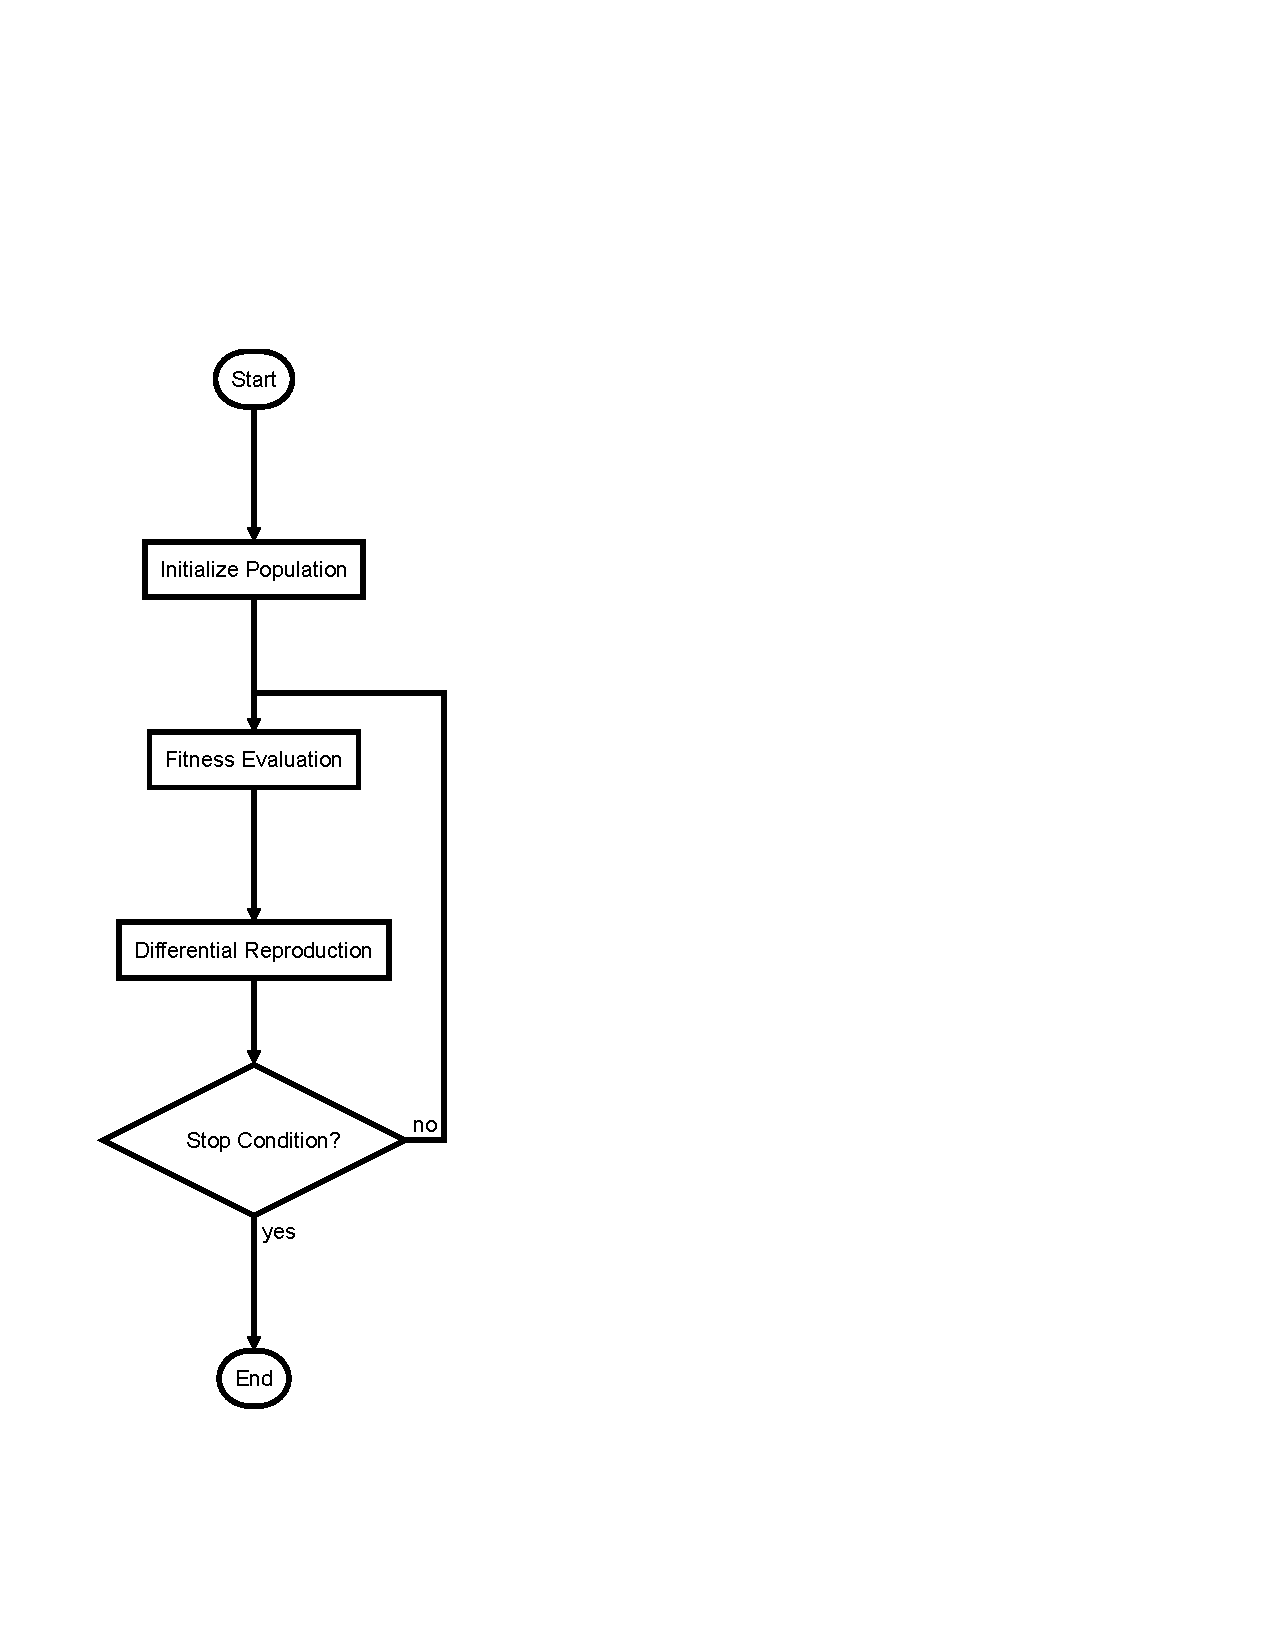
\includegraphics{GeneticAlgorithm.pdf}
	\caption{A high-level view of a genetic algorithm.}
\end{figure}

%% Artificial Neurons
\section{Artificial Neurons}

% TODO: Cite at least one work in this section besides Chalmers, looking for foundational works on ANs and the delta rule and a modern textbook or tutorial or survey paper that covers both 

Artificial neurons are computational elements inspired by the biological neurons found in nature.
An artificial neuron is comprised of a number of weighted input connections, an activation function which implements a response to input, and a number of output connections.

% TODO: Match the font in this figure to the font in the text
\begin{figure}[H]
	\centering
	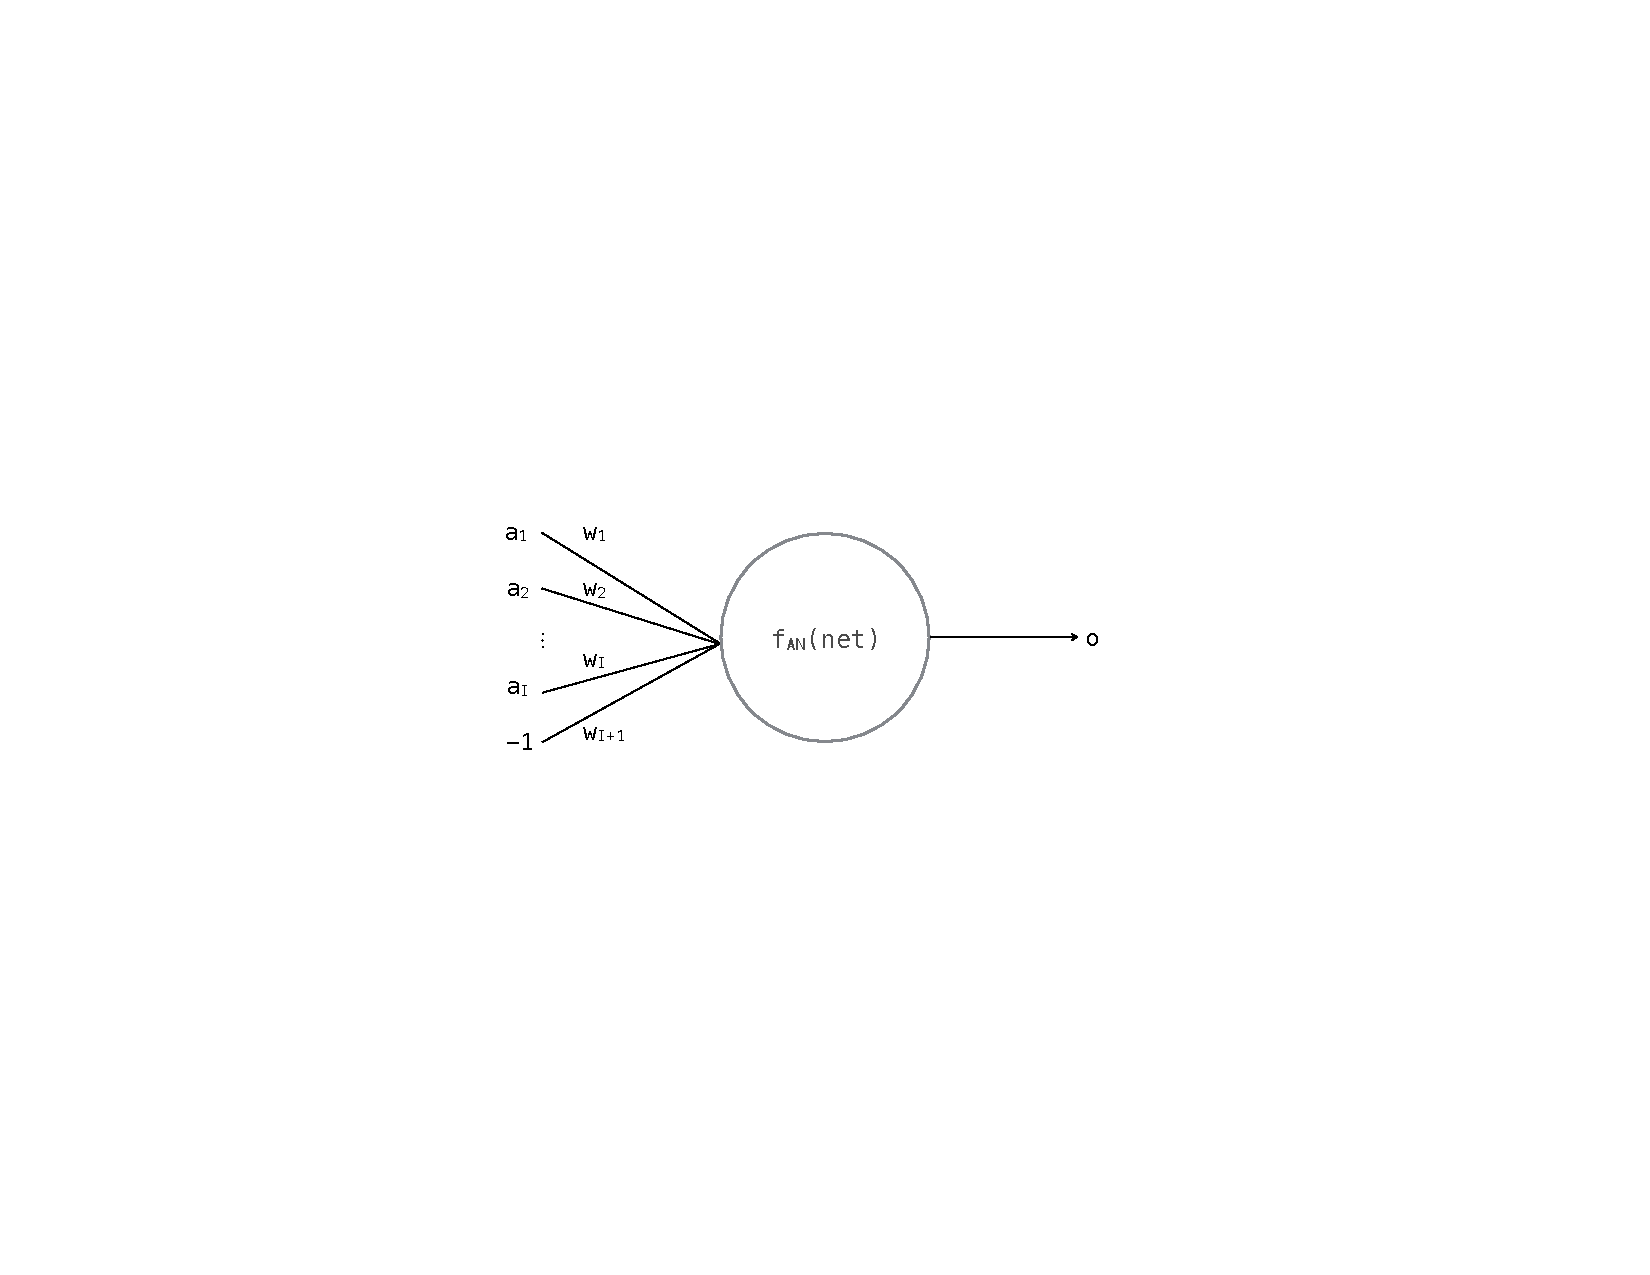
\includegraphics{ArtificialNeuron.pdf}
	\caption{An artificial neuron.}
	\label{fig:neuron}
\end{figure}

Figure \ref{fig:neuron} depicts an artificial neuron with $I$ inputs, one output, and an activation function $f_{AN}$. The neuron receives a vector of $I+1$ input signals, $\mathbf{a}=(a_1, a_2, \ldots, a_I, a_{I+1})$, where $a_{I+1}$ is known as a \emph{bias unit} and always has a value of $-1$.  The input vector is modulated by a weight vector, $\mathbf{w}=(w_1, w_2, \ldots, w_I, w_{I+1})$, where each weight $w_i$ modulates the input signal $a_i$. The neuron computes the net input as the sum of the weighted input signals, giving
\begin{displaymath}
net=\sum_{i=1}^{I+1}a_iw_i.
\end{displaymath}
The output signal, $o$, is then computed by applying the activation function to the weighted input, so that $o=f_{AN}(net)$.

A common choice for $f_{AN}$ is the sigmoid function:

\begin{displaymath}
f_{AN}(net) = \frac{1}{1 + e^{-\lambda net}}
\end{displaymath}
where the parameter $\lambda$ influences the steepness of the function, but usually $\lambda = 1$.

Artificial neurons can be used to compute linearly separable functions without error. This means that, for such a function, there exists at least one threshold value such that the neuron can separate the space of $I$-dimensional input vectors which produce an above-threshold output from those which produce a below-threshold output by an $I$-dimensional hyperplane. This threshold is determined by the bias weight $w_{I+1}$, meaning that the neuron can be used to separate the input vectors for which $net > 0$ from the input vectors for which $net \le 0$.

Learning is a technique by which the weights of an artificial neuron are updated to realize functions given by data.
One type of learning is known as \emph{supervised learning}, where the neuron is provided with a data set, known as the \emph{training set}, consisting of training patterns of input vectors with associated target outputs.
The weights of the neuron are then adjusted until the error between the actual outputs of the neuron and the target outputs in the patterns is minimized.

An example of a supervised learning rule is the so-called \emph{delta rule}.
The delta rule requires the definition of an error function, $\mathcal{E}$, to measure the neuron's error in approximating training targets.
The sum of squared errors is usually used, given by

\begin{displaymath}
\mathcal{E} = \sum_{p=1}^{P_T}(t_p-o_p)^2
\end{displaymath}

where $t_p$ and $o_p$ are the target and actual output for the $p$th pattern, and $P_T$ is the total number of patterns in the training set.

Given a single training pattern, weights are updated using

\begin{displaymath}
w_i(t) = w_i(t - 1) + \Delta w_i(t)
\end{displaymath}
with
\begin{displaymath}
\Delta w_i(t) = \eta(- \frac{\partial \mathcal{E}}{\partial w_i})
\end{displaymath}
where
\begin{displaymath}
\frac{\partial \mathcal{E}}{\partial w_i} = -2(t_p - o_p)\frac{\partial f_{AN}}{\partial net_p}a_{i,p}
\end{displaymath}
and $\eta$ is a constant known as the learning rate, $net_p$ is the net input for pattern $p$, and $a_{i,p}$ is the $i$th input signal in pattern $p$.

The delta rule requires that its activation function $f_{AN}$ is continuous and differentiable;
this is so the gradient of the error can be followed toward lower values, giving the direction in which the weights should be updated.
If we use the sigmoid function for $f_{AN}$ then
\begin{displaymath}
\frac{\partial f_{AN}}{\partial net_p} = o_p(1 - o_p)
\end{displaymath}
giving
\begin{displaymath}
\frac{\partial \mathcal{E}}{\partial w_i} = -2(t_p - o_p)o_p(1 - o_p)a_{i,p}
\end{displaymath}

Artificial neurons are generally connected together into artificial neural networks to perform more sophisticated computation;
however, this work is based closely on the work of Chalmers which considered single neurons in isolation \cite{chalmers-evolution-learning}.

%% Neuroevolution
\section{Neuroevolution}

% Neural network connection strengths, topology, and learning rules can be encoded by strings, meaning they can be evolved by genetic algorithms.
Any feature of an artificial neuron, such as connection weights, activation functions, learning rules, and input features, can be subjected to an evolutionary process after being string-encoded \cite{Yao:1999lp}.
However, this work will focus on the evolution of connection weights and learning rules.

The connection weights of a non-learning neuron can be evolved as the fixed response of that neuron to input.
This is analogous to the evolution of instincts or what we think of as ``hard-wired" behavior.

Alternately, the initial connection weights of a learning neuron can be evolved as the initial behavior which will be modified by the neuron's learning rule.
This can be beneficial for evolving passably fit initial behavior that is then fine-tuned by learning
but it can also be the case that the values of the initial weights are not adaptive and weights are evolved that are effectively random.

Learning rules can be evolved stand-alone by applying them to neurons initialized with random weights in the fitness function.
In this situation the values of the initial weights do not matter because the idea is to evolve learning rules that will converge on a solution that is independent of the values of the starting weights.

The initial connection weights and the learning rules that modify them can be evolved simultaneously.
In this situation, instincts, learning, or a combination of both can be evolved depending on the environment.
This work will examine the outcomes of the simultaneous evolution of connection weights and learning rules under different conditions,
whereas Chalmers examined only the possibility of evolving learning rules.

%% The Evolution of Learning
\section{The Evolution of Learning}

Evolution and learning are both forms of adaptation.
Evolution takes place across generations whereas learning takes places within an individual's lifetime.
Evolution can produce adaptive behaviors such as learning or non-adaptive behaviors such as instincts.

If an environment is sufficiently diverse or dynamic, instinctual behavior is not reasonably adequate for good task performance;
this is because such an environment will invariably present novel tasks to which the instinctual behavior is not well-adapted.

Evolved learning behavior that is scalable and adaptive to unknown or changing situations can be seen in countless species in nature \cite{Shah:2015hs}.

Chalmers \cite{chalmers-evolution-learning} evolved learning rules by encoding the parameters of a template formula as strings, demonstrating that the delta rule for supervised learning can be evolved in certain situations for artificial neurons in static environments.

% TODO: Say more about the work of both Chalmers and Shaw. 
% TODO: Add in mentions (and citations) for several other papers on the evolution of learning.

Shah \cite{Shah:2015hs} similarly demonstrated the evolution of reinforcement learning in changing environments.

%% Nurturing
\section{Nurturing}

\emph{Nurturing} is defined as ``the contribution of time, energy, or other resources by one individual to the expected physical, mental, social, or other development of another individual with which it has an ongoing relationship" \cite{nurturing-definition}.

Nurturing is prevalent in the biological world and can be an important contributing factor to the evolution of learning \cite{nurturing-definition} \cite{eskridge-learning-uncertain-environments}.

% TODO
Nurturing itself can be either instinctive or learned. <Discuss how Leonce, Hoke, and Hougen demonstrated the evolution of instinctive nurturing in robots.>

%TODO
<Include material here on the virtuous cycle that is hypothesized to exist between nurturing and learning.> 

Nurturing can cover the initial costs of a learner and the resulting benefits of learning can be paid forward to the next generation. In this way, nurturing can promote the evolution of learning.

Eskridge \& Hougen \cite{eskridge-learning-uncertain-environments} conducted experiments involving food patch estimation in uncertain environments, and their results demonstrated that nurturing as both social learning and safe exploration can promote the evolution of learning. Shah \cite{Shah:2015hs} demonstrated that nurturing as task simplification can promote the evolution of reinforcement learning in changing environments.

This work explores nurturing as safe exploration in that individuals do not incur fitness penalties for mistakes made during the learning process.

% % Contents of the Thesis
\section{Contents of the Thesis}

The rest of this thesis is organized as follows:
Hypotheses about how nurturing affects the evolution of learning and instincts are detailed in \textbf{Chapter 2}. 
Operational definitions for terms such as ``nurturing" and ``instincts" are introduced in \textbf{Chapter 3}.
Procedures for the experiments examining the effect of nurturing on the evolution of learning and instincts are detailed in \textbf{Chapter 4}.
The experimental results, which demonstrate that nurturing facilitates the evolution of learning, are outlined in \textbf{Chapter 5}. 
The conclusion that nurturing facilitates the evolution of learning is described in \textbf{Chapter 6}. 
Finally, ideas for exploring the interaction between nurturing and the Baldwin effect in future work are described in \textbf{Chapter 7}.

% Hypotheses
\chapter{Hypotheses}

Three factors are considered with respect to their effects on the evolution of learning: the number of tasks, the presence or absence of nurturing, and the possibility of evolving instincts.

Chalmers demonstrated that the likelihood of evolving generalized learning mechanisms is proportional to the number of tasks in the evolutionary environment. When there are few tasks in the evolutionary environment, generalized learning is less likely to evolve.

Given environments like those used by Chalmers, where instincts cannot be evolved, the addition of nurturing alone will have little impact on the evolution of generalized learning because learning is still the only viable strategy in that setup. Therefore, it is expected that the quality of evolved generalized learning mechanisms will remain proportional to the number of tasks and the quality of the learning evolved will be no greater with nurturing than without.

$\mathbf{H_1}$: When only learning rules are evolved, the quality of generalized learning evolved will be proportional to the number of tasks in the evolutionary environment, both with and without nurturing.

$\mathbf{H_2}$: When only learning rules are evolved, the quality of generalized learning evolved will be equal with nurturing and without.

The introduction of the ability to evolve initial network weights alongside learning rules allows for the evolution of ``instincts" as an alternate strategy to learning.
It is expected that higher-quality instincts will evolve for small numbers of evolutionary tasks, but higher-quality learning will evolve as the number of evolutionary tasks increases.
This will be because there will be a smaller number of instinct genes than learning genes to ``tune" to a correct solution for small number of tasks, but because the number of genes required to represent instincts will increase as the number of tasks increases the number of instinct genes will become much larger than the number of learning genes as the number of tasks increases.

$\mathbf{H_3}$: When both initial weights and learning rules are evolved, the quality of instincts evolved will be inversely proportional to the number of tasks in the evolutionary environment, both with and without nurturing.

$\mathbf{H_4}$: When both initial weights and learning rules are evolved, the quality of generalized learning evolved will be proportional to the number of tasks in the evolutionary environment, both with and without nurturing.

It is expected that higher-quality generalized learning will evolve in the nurturing condition than in the non-nurturing condition---and higher-quality instincts will evolve in the non-nurturing condition than in the nurturing condition---because of the costs associated with the learning process in the non-nurturing condition; individuals tend to have low fitness early in their life before they have had the opportunity to learn correct behavior, but in the nurturing condition individuals do not incur fitness penalties for mistakes made early in life.

$\mathbf{H_5}$: When both initial weights and learning rules are evolved, higher-quality instincts will evolve without nurturing than with.

$\mathbf{H_6}$: When both initial weights and learning rules are evolved, higher-quality generalized learning will evolve with nurturing than without.

% Operational Definitions
\chapter{Operational Definitions}

An individual is a candidate solution to the genetic algorithm's fitness function whose characteristics are represented by a chromosome ("Computational Intelligence", pg. 129). In this work, individuals are manifest as artificial neurons. 

A task is a set of input-output patterns, 
[A] where individuals are evaluated by their ability to produce the pattern outputs when activated with the corresponding pattern inputs.
[B] where for each pattern in the task an individual is evaluated on its ability to produce the pattern output when activated with the corresponding pattern inputs.

An environment is a set of tasks by which individuals are assessed.

An individual's lifetime is the period during which it is manifest as an artificial neuron and assessed by the fitness function. Specifically, an individual's lifetime consists of a supervised learning period followed by a final evaluation.

Instincts are to be represented by the genetically encoded initial weights of a neuron. The tasks are independent, so there will need to be a separate set of instinct weights for each task.

Learning is to be represented by the genetically encoded learning rule that is applied to a neuron throughout its lifetime.

For evolved neurons where both initial weights and learning rules are genetically encoded, instincts are measured by removing the learning rule and evaluating the fitness of the neuron in the environment in which it was evolved.
For the same neurons, learning ability is measured by replacing the genetically encoded initial weights with random initial weights and evaluating the fitness of the neuron in the environment in which it was evolved; generalized learning ability is measured by evaluating the fitness of this instinct-removed neuron in an environment different from the one in which it was evolved.

% Don't speak in terms of "mistakes made during learning" because this doesn't make clear that learning fitness is omitted entirely in the nurturing condition
% Instead, note that individuals are more prone to make errors during the training period

[A] By default, mistakes made by a neuron during learning will count against its lifetime fitness; this is the ``non-nurturing" condition.
In the ``nurturing" condition, then, mistakes made by a neuron during learning will not count against its lifetime fitness.

% Is it clear enough that the supervised learning used involves fitness evaluations? 
[B] By default, an individual's lifetime fitness is the average of all fitness evaluations made during learning---when the individual is prone to making mistakes---and the final fitness evaluation that follows learning; this is the ``non-nurturing" condition.
In the ``nurturing" condition, then, an individual's lifetime fitness is simply the result of the final fitness evaluation taken after the individual has had an opportunity to learn correct behavior.

% Procedure
\chapter{Procedure}

%% Genetic Coding of Learning Mechanisms
\section{Genetic Coding of Learning Mechanisms}

The weight update rule for an artificial neuron needs to be based on the components of that neuron which are, as covered in Section 1.2, $a_j$ the activation of the input unit $j$, $o_i$ the activation of the output unit $i$, $t_i$ the training signal on output unit $i$, and $w_{ij}$ the current value of the connection strength from input $j$ to output $i$.

Following Chalmers (1990), the genome encodes a function $F$ such that $\Delta w_{ij} = F(a_j, o_i, t_i, w_{ij})$, where $F$ is a linear function of its four parameters and their six pairwise products. Thus $F$ is determined by specifying ten coefficients.

The genome encodes these ten coefficients, as well as an eleventh ``scale" parameter. That is,
\[
	\Delta w_{ij} = k_0(k_1w_{ij}+k_2a_j+k_3o_i+k_4t_i+k_5w_{ij}a_j+k_6w_{ij}o_i+k_7w_{ij}t_{i}+k_8a_jo_i+k_9a_jt_i+k_{10}o_it_i),
\]
where $k_0$ to $k_10$ are the encoded coefficients.

The portion of the genome which encodes $\Delta w_{ij}$ consists of 35 bits. The first five bits encode the scale parameter $k_0$ such that it can represent the values $0$, $\pm 1/256$, $\pm 1/128$, ..., $\pm 32$, $\pm 64$, via exponential encoding. The first bit encodes the sign of $k_0$ (0: negative, 1: positive), and the next four bits encode the magnitude. If these four bits are interpreted as an integer $j$ between 0 and 15, we have

\[
	|k_0|=
	\begin{cases}
		0 & \text{if $j = 0$}\\
		2^{j-9} & \text{if $j = 1, ..., 15$.}
	\end{cases}
\]

The other 30 bits encode the other ten coefficients in groups of three. The first bit of each group expresses the sign, and the other two bits express a magnitude of 0, 1, 2, or 4 via a similar exponential encoding. If we interpret these two bits as an integer $j$ between 0 and 3, then

\[
	|k_i|=
	\begin{cases}
		0 & \text{if $j = 0$}\\
		2^{j-1} & \text{if $j = 1, 2, 3$.}
	\end{cases}
\]

%% Genetic Coding of Initial Weights
\section{Genetic Coding of Initial Weights}

Initial weights may be evolved alongside learning rules. It would not be meaningful for each chromosome to encode a single set of weights to be used on all tasks, so instead each chromosome simultaneously encodes a distinct set of weights for each task in the evolutionary environment. The weights to be applied to each evolutionary task are encoded in distinct, consistent regions of each chromosome. 

\newcommand{\bitsperweight}{3}
\newcommand{\jlen}{2}
\newcommand{\jmin}{0}
\newcommand{\jmax}{3}
\newcommand{\exponentshift}{4}

Initial weights are encoded using 3 bits each. The first bit is the sign of the weight, and the other two bits express a magnitude of 0, $\frac{1}{8}$, $\frac{1}{4}$, or $\frac{1}{2}$ via an exponential encoding. If we interpret the remaining two bits as an integer $j$ between 0 and 3, then

\[
	|k_i|=
	\begin{cases}
		0 & \text{if $j = 0$}\\
		2^{j-4} & \text{if $j = 1, 2, 3$.}
	\end{cases}
\]

For each task the number of weights encoded is equal to the number of inputs in that task plus one bias weight.

%% Evaluation of Fitness
\section{Evaluation of Fitness}

There are two conditions of evaluation: the ``nurturing" case and the ``non-nurturing" case. During evaluation, each network is first trained for 10 epochs using its learning rule. Following this, the network is evaluated on the same tasks. In the ``nurturing" case the individual's fitness is simply the result of the evaluation, whereas in the ``non-nurturing" case the individual's fitness is the average of evaluation during all training epochs and the final evaluation.

Fitness evaluation for the nurturing case:

(1) Create a network with the appropriate number of input units for the task and a single output unit.

(2) Initialize the connection strengths of the network using the values encoded in the chromosome.

(3) For 10 epochs, cycle through the training exemplars for the task, where for each exemplar:

(3a) propagate input values through the system, yielding output values; then

(3b) adjust the weights of the system according to the formula specified by the weight update rule, on the basis of inputs, output, training signal, and current weights.

(4) At the end of this process, fitness on the task is measured by testing the network on all training exemplars, and dividing the total error by the number of exemplars, and subtracting from 1. This yields a fitness value between 0 and 1.

Fitness evaluation for the non-nurturing case:

(1) Create a network with the appropriate number of input units for the task and a single output unit.

(2) Initialize the connection strengths of the network using the values encoded in the chromosome.

(3) For 10 epochs, cycle through the training exemplars for the task, where for each exemplar:

(3a) test the network on the exemplar and measure the error in the network output; then

(3b) propagate input values through the system, yielding output values, then adjust the weights of the system according to the formula specified by the weight update rule, on the basis of inputs, output, training signal, and current weights.

(4) At the end of this process, test the network on all training exemplars and divide the total error of this test and all tests from step 3a by the total number of tests that occurred, and subtracting from 1. This yields a fitness value between 0 and 1.

Fitness of the chromosome is obtained by evaluating its performance on each of the (typically 20) tasks, and taking the mean fitness over all tasks. In this way every chromosome is assigned a fitness between 0 and 1.

%% Parameters of the Genetic Algorithm
\section{Parameters of the Genetic Algorithm}

% TODO: Describe "segment-wise" crossover used

A fixed population size of 40 is used in all experiments. Following the fitness evaluation process described in Section 4.3, a new population of 40 individuals is created as follows:

(1) Elitist selection is applied, meaning that an exact copy of the individual with the highest fitness in the previous population is inserted into the new population.

(2) Roulette-wheel selection (where an individual's probability of being selected is linearly proportional to its fitness) is used to select 39 individuals from the previous population with replacement (so an individual can be selected more than once), then:

(2a) the first 32 selected individuals are reproduced by gene-wise two-point crossover in pairs to create 32 new individuals which are inserted into the new population;

(2b) the remaining 7 selected individuals are reproduced by cloning to create 7 new individuals which are inserted into the new population.

(3) Each individual in the new population is mutated such that each bit in each chromosome has a 1\% chance of changing.

This cycle of fitness-evaluation and reproduction is repeated for 4000 generations.

Population size: 40
Crossover rate: 0.8
Mutation rate: 0.01
Elitism factor: 1
Number of generations: 4000

%% Post-Evolutionary Evaluation
\section{Post-Evolutionary Evaluation}

Before each evolutionary run, 10 tasks are selected at random from the task pool and designated as ``test tasks,"
and up to 20 tasks are selected at random from the remaining 20 tasks and designated as ``evolutionary tasks."
New evolutionary tasks and test tasks are selected for each repetition of an evolutionary run and between evolutionary runs  nurturing condition and non-nurturing condition .
After each evolutionary run, the chromosome with the highest fitness score in the history of the populations in that run is identified.
From this chromosome, the learning rule bits are isolated and evaluated on the test tasks (using both the nurturing and non-nurturing conditions) and the bits encoding the initial weights are isolated and evaluated on the evolutionary tasks.
Each evolutionary run is repeated 30 times.

% Results
\chapter{Results}

%% Results of Initial Evolutionary Runs
\section{Results of Initial Evolutionary Runs}

\begin{figure}[H]
	\centering
	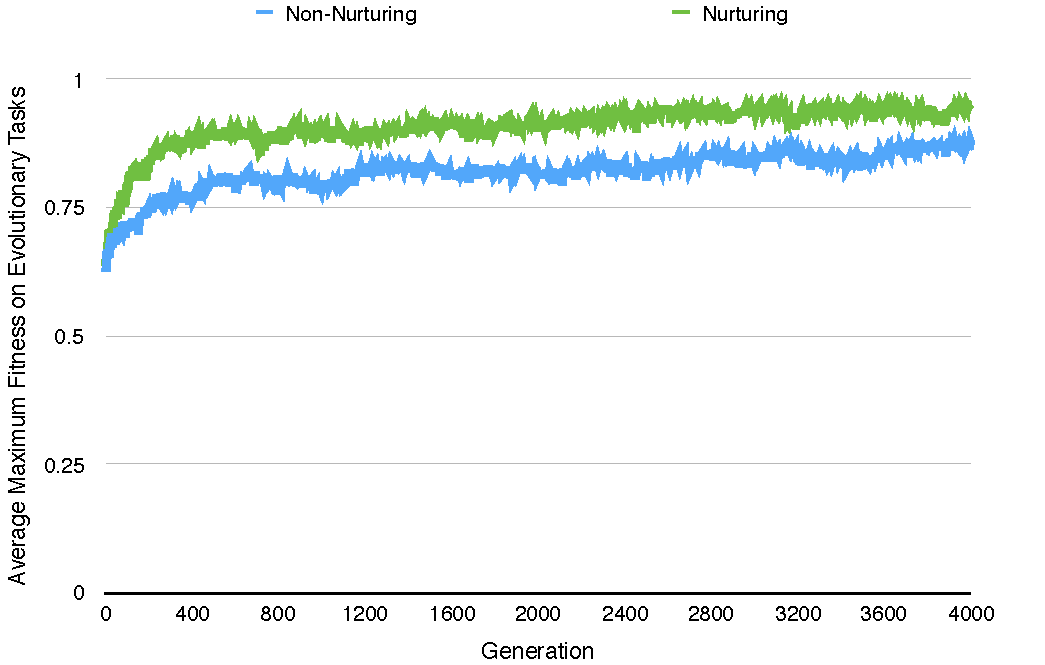
\includegraphics{ChalmersEvolution.pdf}
	\caption{The maximum fitness for populations evolved using 20 tasks under the nurturing and non-nurturing conditions.}
\end{figure}

% TODO: Add plot of best individuals to serve as learning test plot

% The learning generalization test with nurturing
\begin{figure}[H]
	\centering
	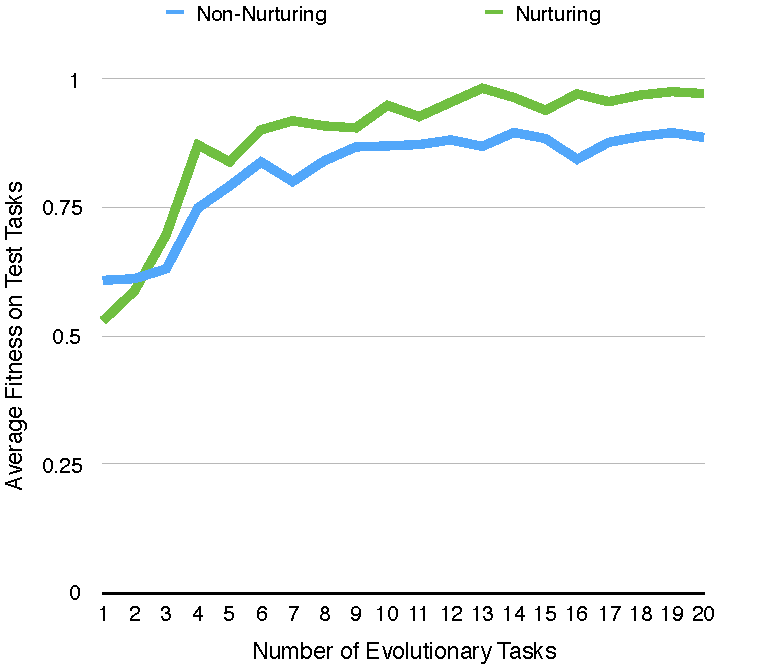
\includegraphics{ChalmersLearningTest.pdf}
	\caption{The average generalized learning capabilities for the best individuals evolved under the nurturing and non-nurturing conditions.}
\end{figure}

%% Fitness Test
\section{Intra-Learning and Post-Learning Fitness Test}

The best individual is re-evaluated on the evolutionary tasks using both the nurturing and non-nurturing conditions (recall that it is evaluated using only one of these conditions during evolution).

Under both conditions it is clear that the objective function becomes more difficult to satisfy as the number of evolutionary tasks increases. 

Individuals evolved using the non-nurturing condition perform better when re-evaluated using the intra-learning fitness test/non-nurturing condition than when using the post-learning test/nurturing condition, and individuals evolved using the nurturing condition perform better when re-evaluated using the post-learning test/nurturing condition than when using the intra-learning test/non-nurturing condition.

\begin{figure}[H]
	\centering
	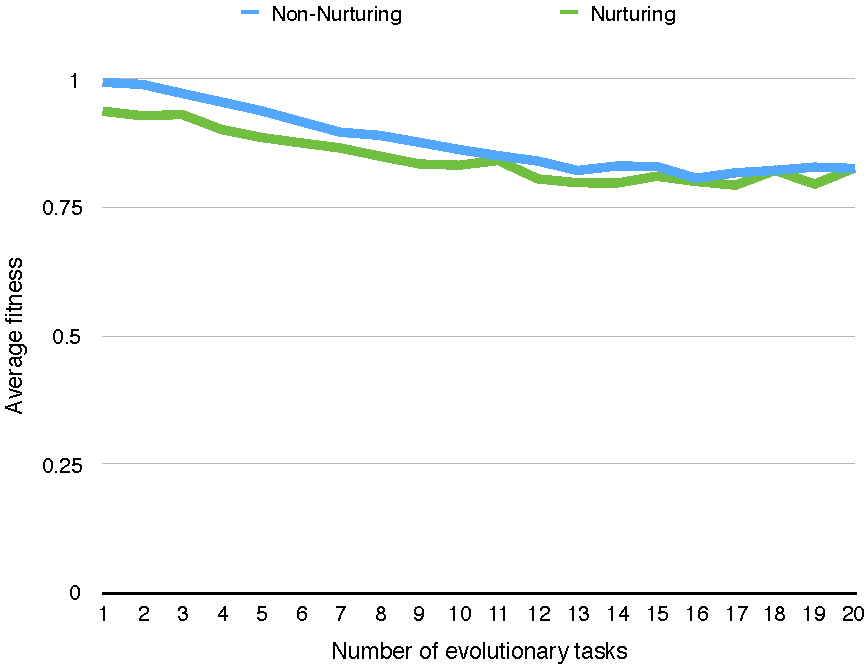
\includegraphics{NonNurturingFitnessTestPlot.pdf}
	\caption{Intra-learning/non-nurturing fitness test on evolutionary tasks for individuals evolved under the nurturing and non-nurturing conditions.}
\end{figure}

\begin{figure}[H]
	\centering
	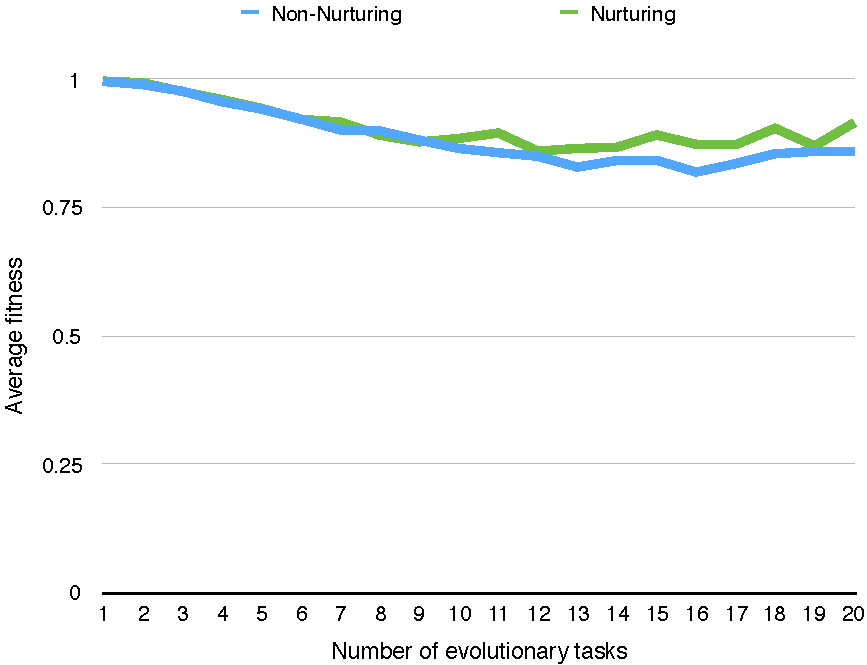
\includegraphics{NurturingFitnessTestPlot.pdf}
	\caption{Post-learning/nurturing fitness test on evolutionary tasks for individuals evolved under the nurturing and non-nurturing conditions.}
\end{figure}

%% Network Test
\section{Pre-Learning Test}

The portion of the chromosome that encodes the initial weights is isolated and evaluated on the evolutionary tasks by initializing a network with the encoded weights, with the intention of determining the contribution to the fitness of the whole chromosome of just the portion of the chromosome that encodes the initial weights.

Networks evolved using the non-nurturing condition performed better on this evaluation than networks evolved using the nurturing condition, suggesting that instincts (initial weights) make a larger contribution to fitness in the non-nurturing case than in the nurturing case.
% TODO: Suggest that learning plays a somewhat less important role in the non-nurturing case?

\begin{figure}[H]
	\centering
	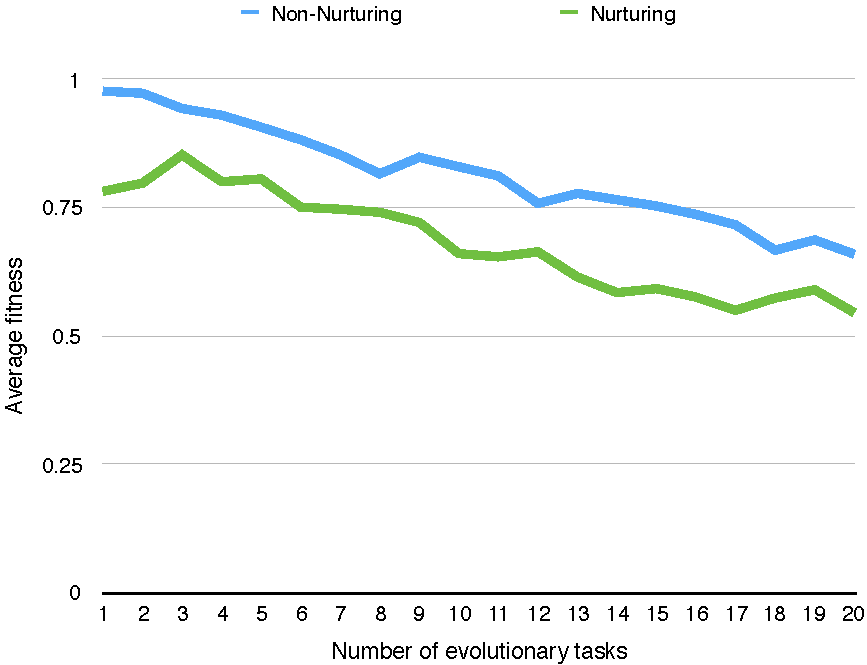
\includegraphics{NetworkTestPlot.pdf}
	\caption{Instinct test on evolutionary tasks for individuals evolved under the nurturing and non-nurturing conditions.}
\end{figure}

%% Learning Improvement
\section{Learning Improvement}

To determine the average amount of useful learning that evolves for a given number of tasks we can examine the difference between the post-learning fitness and the pre-learning (instinctive) fitness.
This is because the pre-learning fitness is the individual's fitness before it learns, whereas the post-learning fitness is an individual's fitness after it learns.

As shown in Figure 4.4, the improvement in fitness due to learning increases as the number of evolutionary tasks increases. This suggests that learning becomes an increasingly important evolutionary strategy as the environment becomes more varied.

\begin{figure}[H]
	\centering
	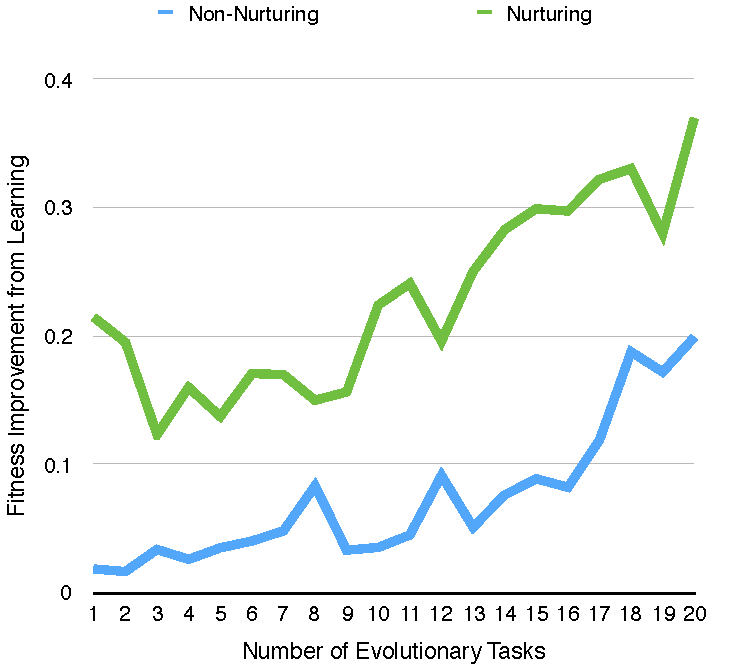
\includegraphics{LearningImprovementPlot.pdf}
	\caption{The difference between evolutionary fitness and network fitness for individuals evolved under the nurturing and non-nurturing conditions.}
\end{figure}

%% Learning Test
\section{Weight-Generalization Learning Test}

The portion of the chromosome that encodes the learning rule is isolated and evaluated on the evolutionary tasks by initializing a network with random weights and the encoded learning rule, with the intention of determining the contribution of the portion of the chromosome that encodes the learning rule to the fitness of the whole chromosome.

In both evaluation conditions, the learning rule evolved under the nurturing condition performed better than the learning rule evolved under the non-nurturing condition, suggesting that the learning rule makes a larger contribution to fitness under the nurturing condition than it does under the non-nurturing condition.
% TODO: Suggest that learning plays a somewhat more important role in the nurturing case?

\begin{figure}[H]
	\centering
	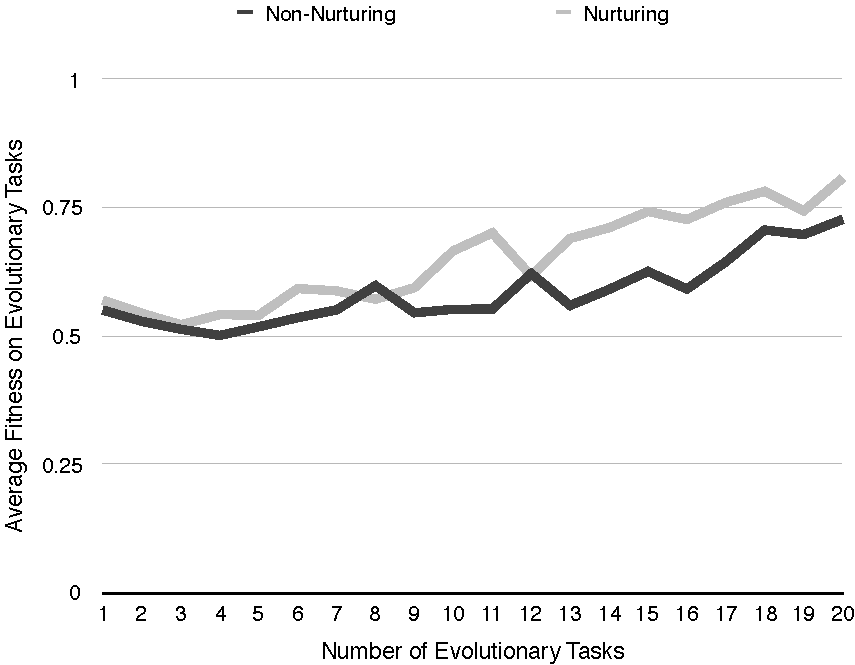
\includegraphics{NonNurturingLearningTestPlot.pdf}
	\caption{Random-start, intra-learning/non-nurturing learning test on evolutionary tasks for individuals evolved under the nurturing and non-nurturing conditions.}
\end{figure}

\begin{figure}[H]
	\centering
	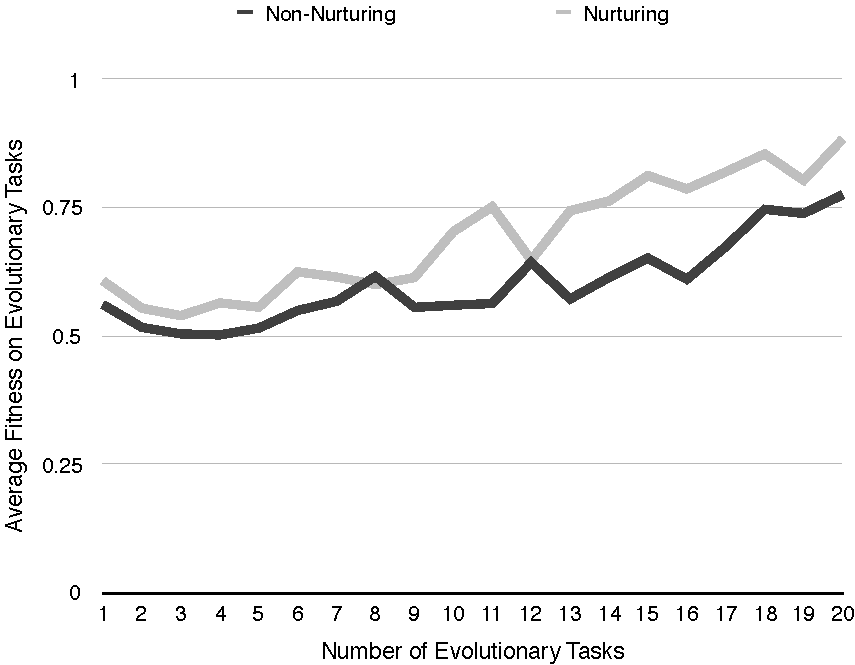
\includegraphics{NurturingLearningTestPlot.pdf}
	\caption{Random-start, post-learning/nurturing learning test on evolutionary tasks for individuals evolved under the nurturing and non-nurturing conditions.}
\end{figure}

%% Task Generalization Learning Test
\section{Task Generalization Learning Test}

The portion of the chromosome which encodes the learning rule is isolated and evaluated on the test tasks by initializing a network with random weights and the encoded learning rule, with the intention of determining the capacity for generalized learning that was evolved.

In both evaluation conditions, the learning rule evolved under the nurturing condition performed better than the learning rule evolved under the non-nurturing condition, suggesting that better generalized learning is more likely to evolve under the nurturing condition.

\begin{figure}[H]
	\centering
	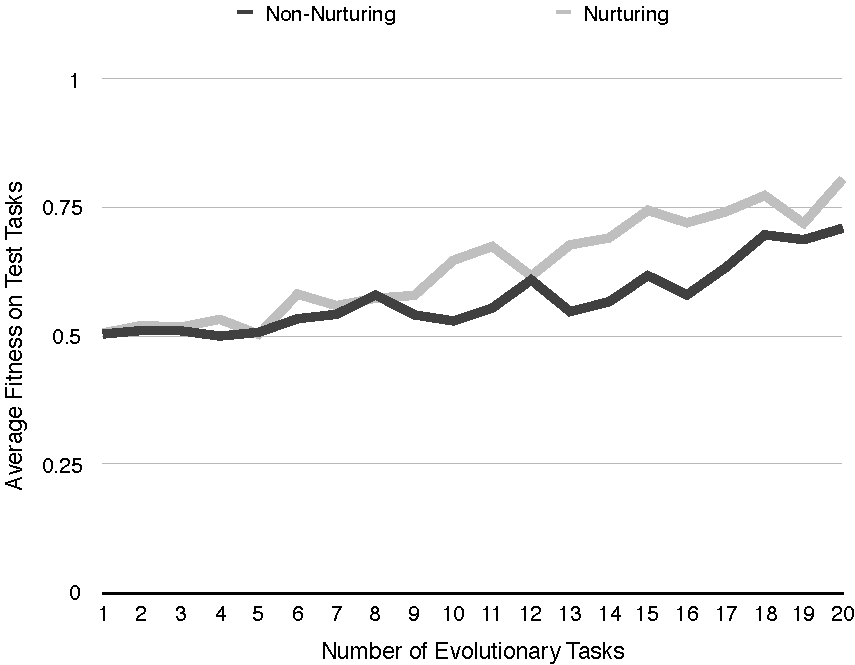
\includegraphics{NonNurturingGeneralizationTestPlot.pdf}
	\caption{Non-nurturing generalization test on test tasks for individuals evolved under the nurturing and non-nurturing conditions.}
\end{figure}

\begin{figure}[H]
	\centering
	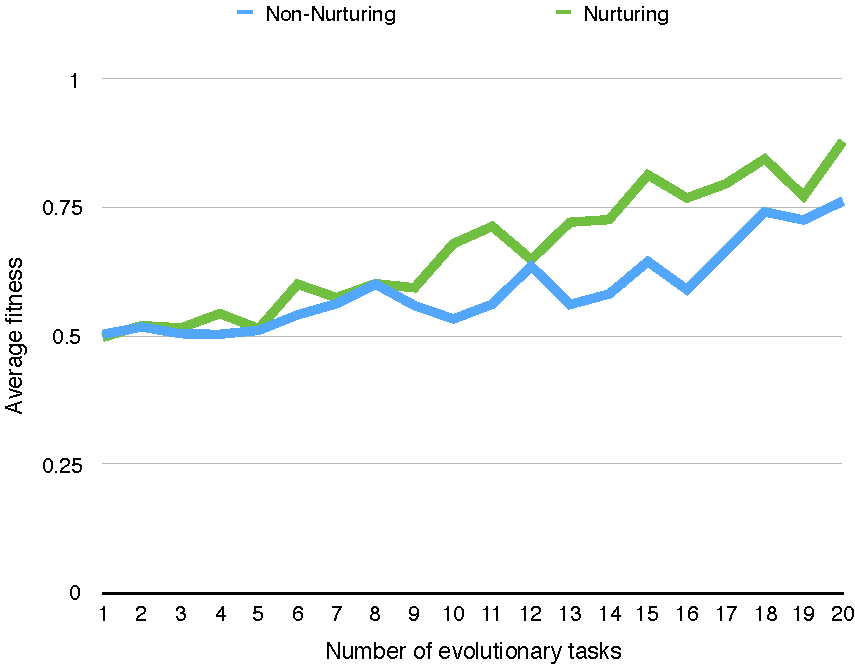
\includegraphics{NurturingGeneralizationTestPlot.pdf}
	\caption{Nurturing generalization test on test tasks for individuals evolved under the nurturing and non-nurturing conditions.}
\end{figure}

% Conclusions
\chapter{Conclusions}

The impact of varying the nurturing condition alone was insignificant; fitnesses measured under the nurturing condition were generally higher than those measured under the non-nurturing condition, but this is to be expected because of the additional fitness penalties imposed by the non-nurturing condition.

When instincts and learning were allowed to evolve alongside each other, it was found that instinct-based solutions were more likely to evolve for small numbers of evolutionary tasks, but that learning became more likely to evolve as the number of evolutionary tasks increased.

By varying the nurturing condition when instincts were allowed to evolve alongside learning, it was found that instinct-based solutions were more likely to evolve under the non-nurturing condition whereas learning was more likely to evolve under the nurturing condition.

% Future Work
\chapter{Future Work}

%% The Baldwin Effect
\section{The Baldwin Effect}

Baldwin (1896) argued that learning accelerates evolution because suboptimal individuals increase their baseline fitness by acquiring more adaptive characteristics during life. 
Lifetime learning often involves a cost because the individual may be at risk at an early stage of its life or it may modify its behavior in ways that are not functional for its survival.
Baldwin suggested that evolution tends to select individuals that are born with some of the useful features that would otherwise be learned.
However, a consequence of this effect is that learned features may gradually become assimilated into the genotype and reduce the role of learning;
this is not necessarily a good effect if it is desirable for the individuals to retain the ability to learn after the completion of the evolutionary process. \cite{Floreano:2008wv} 

Nurturing can reduce the evolutionary costs of learning and thus may be able to inhibit the Baldwin effect.
Inhibiting the Baldwin effect may result in evolved individuals that have greater adaptive capabilities.

\bibliography{Bibliography}{}
\bibliographystyle{plain}

\makebackmatter
\end{document}